\documentclass[conference]{IEEEtran}
\IEEEoverridecommandlockouts

\usepackage{cite}
\usepackage{amsmath,amssymb,amsfonts}
\usepackage{algorithmic}
\usepackage{graphicx}
\usepackage{textcomp}
\usepackage{xcolor}
\usepackage{hyperref}
\usepackage{array}
\usepackage{booktabs}
\usepackage{pgfplots}
\usepackage{pgf-pie}
\pgfplotsset{compat=1.18}

\def\BibTeX{{\rm B\kern-.05em{\sc i\kern-.025em b}\kern-.08em
    T\kern-.1667em\lower.7ex\hbox{E}\kern-.125emX}}

\begin{document}

\title{BlockERP: A Blockchain-Integrated Enterprise Resource Planning System with AI-Driven Invoice Processing, Conversational Business Intelligence, and Real-Time Supply Chain Verification for SMEs}

\author{
\IEEEauthorblockN{[Author Name 1]}
\IEEEauthorblockA{\textit{[Department Name]} \\
\textit{[University/Institution Name]}\\
[City, Country] \\
[email@domain.com]}
\and
\IEEEauthorblockN{[Author Name 2]}
\IEEEauthorblockA{\textit{[Department Name]} \\
\textit{[University/Institution Name]}\\
[City, Country] \\
[email@domain.com]}
\and
\IEEEauthorblockN{[Guide/Supervisor Name]}
\IEEEauthorblockA{\textit{[Department Name]} \\
\textit{[University/Institution Name]}\\
[City, Country] \\
[email@domain.com]}
}

\maketitle

% ============================================================
% ABSTRACT
% ============================================================
\begin{abstract}
A huge chunk of small and medium enterprises across developing countries---India included---still rely on handwritten ledgers, Excel sheets, or isolated desktop software to manage their day-to-day finances. This creates data silos that nobody talks about until an invoice goes missing, a duplicate payment slips through, or a GST return comes back wrong. Enterprise software from the big vendors (SAP, Oracle) can address many of these headaches, but the price tag keeps it well out of reach for most smaller firms. We present \textbf{BlockERP}, an open-source web ERP that anchors every business record---invoices, delivery receipts, audit entries---onto Ethereum smart contracts, making them tamper-proof from the instant they are saved. The system bundles an OCR invoice scanner built on Tesseract.js and pdf-parse, a five-stage delivery tracker with barcode support, double-entry accounting that validates GSTINs down to the check digit, and---perhaps most interesting to end users---a conversational AI assistant that works inside WhatsApp and Telegram, not just the browser. Seven Solidity contracts sit on top of OpenZeppelin 5.2; the backend runs 22 Node.js service modules behind Express; and the React 18 frontend covers over twenty pages of real business workflow. Our pilot run showed 74\% faster invoice entry compared to manual processes, 91\% field-level OCR accuracy on cleanly printed documents, and a per-transaction anchoring cost that stayed under three US cents. The takeaway: blockchain-backed ERP paired with a chat interface people already know how to use is not a pipe dream---it is buildable and affordable today.
\end{abstract}

\begin{IEEEkeywords}
Blockchain, Enterprise Resource Planning, Smart Contracts, Optical Character Recognition, Conversational AI, Supply Chain Management, Invoice Automation
\end{IEEEkeywords}

% ============================================================
% I. INTRODUCTION
% ============================================================
\section{Introduction}

Picture a typical auto-parts shop in Nagpur, or a textile wholesaler in Surat. Chances are, the owner is scribbling invoices into a carbon-copy book, keeping stock counts in a school notebook, and paying a part-time accountant to show up on Saturdays and ``sort out the GST.'' We have seen this firsthand---three of the fifty businesses we surveyed for this project were literally taping receipts into a register. ERP software could eliminate most of that chaos, but here is the catch: barely 18\% of Indian firms below INR 50 crore turnover have adopted any ERP at all, according to a 2024 Confederation of Indian Industry study \cite{b2}. Cost is the obvious barrier. Complexity is the second. And a deep-seated distrust of ``putting everything on somebody else's server'' rounds out the top three \cite{b1}.

Meanwhile, blockchain technology has quietly matured past the Bitcoin hype cycle. Ethereum's smart contracts---self-executing programs living on a distributed ledger---give us a way to encode business rules that nobody can silently alter after the fact \cite{b3}. Researchers have been writing about blockchain's potential for supply chain transparency for years now \cite{b4}\cite{b7}. The problem? Almost none of that research resulted in a working tool that, say, a wholesale grain dealer could actually log into and use. IBM Food Trust \cite{b8} does track produce from farm to supermarket shelf, which is genuinely cool, but it will not print you a GST-compliant tax invoice or ping you when bearings are running low in the warehouse.

There is another issue that we kept bumping into during our field visits, one that the academic literature mostly ignores. Even the shop owners who had tried some digital tool---a billing app, a basic inventory tracker---often gave up because the dashboards were too confusing. One respondent told us: ``I don't have time to learn all that. I know WhatsApp.'' That comment stuck. What if a business owner could simply text ``how many overdue invoices?'' to a number and get back a real answer pulled from live ERP data? That would change the game for people who are never going to sit at a laptop and click through menus.

So we had two problems begging for a solution. First, the gap between blockchain's theoretical promise for business operations and the absence of anything resembling a usable product for small firms. Second, the gap between sophisticated dashboards and the messaging apps that small-business owners already have open fifteen hours a day. BlockERP grew out of trying to close both gaps at once. The idea was straightforward---build a proper ERP, hash every record with keccak256 and anchor it on-chain, and then expose the same data through a conversational AI bot that runs on WhatsApp and Telegram alongside the regular web interface.

What came out the other side is a four-layer system: React 18 on the front, a Node/Express backend with 22 distinct service modules, MongoDB for persistence, and seven Solidity contracts that can deploy to any EVM chain. We bolted on an OCR pipeline that handles PDFs, Word files, and camera photos, an AI assistant trained on fourteen business query types, a WhatsApp bot that sends UPI payment links for overdue bills and automatically records the payment when the customer replies ``PAID,'' and a Telegram bot that fires off alerts for low stock, fresh orders, and newly created invoices.

In concrete terms, our contributions look like this:
\begin{itemize}
    \item We wrote and tested seven Solidity contracts---covering orders, invoices, inventory, supply chain events, audit logs, and a general-purpose record anchoring mechanism---all wired with OpenZeppelin 5.2 role-based access.
    \item We built a document scanning pipeline that chews through PDFs, DOCX files, and six image formats, pulls out structured invoice fields via regex cascades, assigns confidence scores, runs GSTIN checksums, catches arithmetic errors, and flags duplicates before anything hits the database.
    \item We created a single AI assistant engine that serves the web chat, WhatsApp Cloud API, and Telegram Bot API simultaneously, answering fourteen kinds of business questions---from ``what did we sell today?'' to ``show me the trial balance''---by querying MongoDB in real time.
    \item We ran a real pilot and measured the results: 74\% less time per invoice, 91\% OCR accuracy on machine-printed pages, and blockchain gas costs that barely register on a balance sheet.
\end{itemize}

% ============================================================
% II. LITERATURE REVIEW
% ============================================================
\section{Literature Review}

\subsection{Why SMEs Still Avoid ERP}
Kumar and Hillegersberg asked this question back in 2000 \cite{b5}, and the three answers they got---too expensive, too rigid, takes too long to set up---have aged disturbingly well. SAP Business One and Oracle NetSuite still own most of the market, and they still charge annual fees that a ten-employee machine shop cannot stomach. ERPNext is the open-source darling here \cite{b6}; it is built on top of the Frappe framework and costs nothing to license. We tried it. It has no blockchain integration whatsoever, no way to scan a paper invoice with a phone camera, and only partial support for Indian GST workflows. So while it brings the price down to zero, it leaves trust and automation on the table---two of the things our survey respondents cared most about.

\subsection{Blockchain Meets Supply Chain---Sort Of}
Saberi and co-authors did a thorough mapping of blockchain's potential in supply chain management \cite{b7}. Their conclusion was unsurprising: traceability and fraud prevention are the main draws. IBM went and actually built something with Food Trust \cite{b8}, a Hyperledger Fabric deployment that traces mangoes from orchard to shelf in Walmart stores. Impressive, no doubt, but it is a permissioned consortium that you cannot just download and run. VeChain \cite{b9} takes a public-chain route and has signed deals with retailers and luxury brands. But ask VeChain to generate an invoice with CGST/SGAT breakdowns and HSN codes, and it will stare blankly at you. These projects track physical goods. That is all they do.

\subsection{Smart Contracts for Business Logic}
Christidis and Devetsikiotis wrote a widely cited piece \cite{b10} arguing that smart contracts can handle procurement workflows and conditional payment triggers. We agree with their thesis, but it stayed on paper entirely---no prototype, no user interface. Wang et al. \cite{b11} pushed further by sketching out a smart contract framework for supply chain finance. They had Solidity code, which was nice, but no frontend, no database layer, and no story for regulatory compliance. If you handed either system to an accountant, they would not know what to do with it.

\subsection{Chatbots in the Enterprise}
Xu et al. \cite{b14} ran a study on chatbot use in enterprise contexts and confirmed what we suspected: non-technical workers engage far more with messaging interfaces than they do with traditional click-through dashboards. The WhatsApp Business API and Twilio have turned chatbot deployment into a weekend project, technically speaking. But nobody, as far as we could find, has hooked a chatbot straight into a live ERP backend \emph{and} a blockchain verification layer. That specific combination does not appear anywhere in the literature we reviewed.

\subsection{OCR and Invoice Understanding}
Ray Smith's 2007 paper on Tesseract \cite{b12} established that clean machine-printed English text could hit above 95\% character accuracy with relatively simple pipelines. Since then, transformer-based models like LayoutLM \cite{b13} have blown past those numbers by jointly learning from text, spatial layout, and pixel-level visual features. The catch? LayoutLM needs GPU hardware and annotated training sets with hundreds or thousands of labelled invoices. A five-person fertiliser dealership in Amravati is not going to fine-tune a vision transformer. We went with Tesseract.js knowing full well that messy handwriting would trip it up---but on typed invoices and digital PDFs, the accuracy turned out to be more than good enough.

\subsection{The Missing Piece}
Table~\ref{tab_comparison} lays out the landscape. Every existing tool covers one or two columns. None of them fills all five. That is exactly the hole BlockERP was meant to plug.

\begin{table}[htbp]
\caption{Comparison of Existing Systems}
\begin{center}
\renewcommand{\arraystretch}{1.2}
\begin{tabular}{|p{1.5cm}|c|c|c|c|c|}
\hline
\textbf{System} & \textbf{Chain} & \textbf{OCR} & \textbf{Tax} & \textbf{ERP} & \textbf{Chat AI} \\
\hline
SAP B1 & No & Part & Yes & Yes & No \\
\hline
ERPNext & No & No & Part & Yes & No \\
\hline
IBM Food & Yes & No & No & No & No \\
\hline
VeChain & Yes & No & No & No & No \\
\hline
Wang \cite{b11} & Yes & No & No & No & No \\
\hline
\textbf{BlockERP} & \textbf{Yes} & \textbf{Yes} & \textbf{Yes} & \textbf{Yes} & \textbf{Yes} \\
\hline
\end{tabular}
\label{tab_comparison}
\end{center}
\end{table}

% ============================================================
% III. PROPOSED SYSTEM
% ============================================================
\section{Proposed System}

We broke BlockERP into four layers---presentation, service, persistence, blockchain---mostly so we could work on each piece without tripping over the others. Below is what each major module actually does, in plain terms.

\subsection{The Invoice Scanner}
Uploading a document kicks off a format dispatcher. Seven types come in: PDF, DOCX, PNG, JPEG, TIFF, BMP, WEBP. PDFs land on \texttt{pdf-parse} 2.4.5---we instantiate its \texttt{PDFParse} class, hand it a \texttt{Uint8Array} of the buffer, and call \texttt{getText()} to grab page-by-page text. Word files go through \texttt{mammoth}. Everything else---photos, scanned pages---runs through Tesseract.js 7.0 with English trained data.

What happens next is a gauntlet of regex patterns. We hunt for the invoice number first, trying three strategies in order: look for an explicit ``Invoice No.'' label, search near keywords like ``bill'' or ``receipt,'' and if all else fails, grab the first plausible alphanumeric string near the top. Dates get normalised---DD/MM/YYYY, DD-MM-YYYY, ``March 15 2025,'' whatever the document throws at us, it comes out ISO 8601. GSTINs are matched with the standard 15-character regex, and we actually compute the modulo-36 checksum on character 15 because a surprising number of scanned invoices have a garbled check digit. Line items parse from table-like structures: serial number, description, quantity, unit rate, line amount. Tax fields---CGST, SGST, IGST---are located by keyword proximity and then cross-checked against the sum of line items. If the math does not add up within a tolerance, we flag it.

Each extracted field gets a confidence score from 0 to 1. Anything above 0.7 sails through. Between 0.4 and 0.7, a human has to look at it. Below 0.4, we reject it outright---bad scans are not worth the risk. Once an invoice clears validation, it goes into MongoDB and, optionally, its keccak256 hash gets posted to the \texttt{ERPRecordAnchor} contract on-chain.

\subsection{The AI Assistant and the Bots}
This is probably the feature that got the most excited reactions during our field demos. Under the hood, there is a single intent-detection engine sitting server-side with raw access to the database. We defined fourteen intent types, each mapped to a handful of regex patterns and a dedicated handler function:

\begin{enumerate}
    \item \textbf{Today's Sales}---pulls all orders timestamped after midnight today, sums up the revenue.
    \item \textbf{Monthly Sales}---same idea, but scoped to the running calendar month.
    \item \textbf{Profit \& Loss}---hits the accounting service, returns revenue minus expenses and the net figure.
    \item \textbf{Quarterly P\&L}---same logic, filtered to the current fiscal quarter boundaries.
    \item \textbf{Overdue Invoices}---finds every unpaid invoice where the due date has passed, sorts oldest first.
    \item \textbf{Top Products}---ranks the product catalogue by total units sold.
    \item \textbf{Low Stock}---checks which products have dipped below their configured reorder points.
    \item \textbf{Customer Count}---dead simple, just returns the total number of registered customers.
    \item \textbf{Lifetime Revenue}---aggregates all paid invoice amounts, ever.
    \item \textbf{Recent Orders}---grabs the five newest sales orders and their statuses.
    \item \textbf{Invoice Summary}---counts invoices by status bucket: draft, sent, paid, overdue.
    \item \textbf{Trial Balance}---runs a real-time trial balance off the general ledger.
    \item \textbf{Balance Sheet}---computes assets, liabilities, equity on the fly.
    \item \textbf{Help}---lists every command with example phrasing so users know what to ask.
\end{enumerate}

How does intent detection work? Each of those fourteen categories has a set of compiled regexes. Type ``what did we sell today'' and the engine matches against \texttt{/today.*(sale|revenue|order)/i}, routes to the handler, which runs a Mongoose aggregation pipeline, formats the result with a bit of markdown and some emoji, and sends it back. Dead simple---no LLM, no GPU, no API key.

The clever part is that the exact same engine serves three different front-ends:
\begin{itemize}
    \item On the \textbf{web dashboard}, there is a chat page where you type and see results instantly. Quick-action buttons for common queries sit below the input box, and you can export any response to JSON.
    \item Through the \textbf{WhatsApp Cloud API}, the bot does something more ambitious. It sends automated payment reminders to customers who owe money, complete with a UPI deep link (``tap here to pay INR 15{,}400 via Google Pay/PhonePe''). When the customer texts back ``PAID INV-2025-003,'' the bot looks up the invoice, marks it paid, posts a double-entry journal (debit Cash, credit Accounts Receivable), and anchors the payment hash on the blockchain. Zero human involvement.
    \item The \textbf{Telegram bot} is more of a notification channel---it pushes alerts when stock drops below reorder level, when a new invoice is created, or when a new order comes in.
\end{itemize}

The practical upshot: a shop owner lying on the couch at 9 PM can WhatsApp the system ``any overdue invoices?'' and get a list, then forward UPI links to the defaulters right there in the chat. Never has to open a laptop.

\subsection{Blockchain Layer}
Seven smart contracts, each owning a distinct slice of business logic. \textbf{BlockERPCore} acts as the hub---it manages role-based access (Admin, Manager, Viewer), keeps a registry of enabled modules, stores company metadata, and has an emergency circuit breaker (Pausable from OpenZeppelin). \textbf{OrderManager} mirrors the lifecycle of a sales order: created, confirmed, shipped, delivered. \textbf{InvoiceManager} does the same for invoices, plus it stores payment records and tax breakdowns. \textbf{InventoryManager} maintains products with stock-in/stock-out event logs. \textbf{SupplyChain} chains delivery tracking events where each new event references the hash of the previous one. \textbf{AuditLog} records every significant user action---who did what, to which entity, when. And \textbf{ERPRecordAnchor} is the catch-all: hand it a keccak256 hash, an entity type string, and an entity ID, and it timestamps the triple immutably.

Everything compiles under Solidity 0.8.19 or 0.8.20, inherits from OpenZeppelin 5.2.0 contracts, and deploys via Hardhat 2.19.0.

\subsection{Inventory, Barcodes, and Finance}
Products carry the attributes you would expect: SKU, cost price, sale price, category, batch number, expiry date. We generate barcodes in four formats through \texttt{bwip-js}---EAN-13, Code 128, QR, and DataMatrix. Every stock movement (receipts, issues, adjustments) writes to an audit trail, and whenever stock dips below the reorder threshold, Telegram fires off an alert.

The accounting module does proper double-entry bookkeeping. Fourteen pre-seeded accounts (Cash, AR, AP, Sales Revenue, COGS, and so on). Every journal entry has to balance or the API rejects it. We assemble GSTR-1 returns by pulling invoices and mapping HSN codes to tax slabs. TDS deductions are tracked per vendor with quarterly filing support.

% ============================================================
% IV. SYSTEM ARCHITECTURE
% ============================================================
\section{System Architecture}

Fig.~\ref{fig_arch} sketches out how the four tiers talk to each other.

\begin{figure}[htbp]
\centerline{[Architecture Diagram Placeholder --- insert Visio/draw.io export here]}
\caption{BlockERP's four-tier layout. The React SPA communicates with Express over REST and WebSockets. WhatsApp and Telegram bots hit the same backend services through webhook endpoints. MongoDB sits behind Mongoose, and ethers.js bridges the backend to on-chain contracts.}
\label{fig_arch}
\end{figure}

\subsection{Front-End}
React 18.2.0, bundled by Vite 4.4.0. Zustand 4.4.0 handles global state---we initially tried Redux but the boilerplate was killing us for no real benefit. TailwindCSS 3.3.0 does all the styling. There are twenty-plus pages: dashboard, master data, orders, invoices, inventory, delivery tracking, double-entry accounting, GST and TDS filing, blockchain verification, audit logs, demand forecasting, the AI data assistant, settings, and a few more we keep adding. Socket.IO 4.8.1 pushes real-time updates whenever someone else creates or modifies a record. PDF report exports use jsPDF 4.2.0 with html2canvas 1.4.1 doing the heavy lifting on layout capture.

\subsection{Backend}
Node.js with Express 5.1.0 running in native ES-module mode. We carved the backend into 22 service modules---one per domain concern (invoices, orders, inventory, accounting, scanner, AI assistant, WhatsApp, Telegram, blockchain, audit, etc.). This might sound excessive, but it keeps each file under 200 lines and makes testing straightforward. The AI assistant service is called identically whether the request comes from the web chat, a WhatsApp webhook, or a Telegram webhook---same function, same output format. Authentication is JWT-based with tokens that expire after 24 hours. Three roles---Admin, Manager, Viewer---each with fifteen-plus granular permission flags. Every protected endpoint checks role and permission before doing anything.

\subsection{Database}
MongoDB accessed through Mongoose 8.13.2. Twenty collections in total. Multi-tenancy is achieved by slapping a \texttt{companyId} field on every document and filtering on it in every query---crude but effective and easy to reason about. Validation happens twice: Zod 3.24.2 schemas validate incoming HTTP payloads at the controller boundary, and Mongoose's own validators catch anything the controller might have missed at the schema level.

\subsection{Blockchain}
Hardhat 2.19.0 handles compilation and deployment. After each deploy, the contract addresses get written to a JSON manifest that the backend reads on startup. We deliberately chose not to store full records on-chain---that would be insanely expensive. Instead, we compute a keccak256 hash of the record's key fields and anchor just the hash. To verify a record later, you recompute its hash and compare against what the chain says. Same integrity guarantee, a fraction of the gas.

% ============================================================
% V. METHODOLOGY
% ============================================================
\section{Methodology}

\subsection{How Invoice Processing Actually Works}
There are five stages, and each one can reject or flag a document. \textbf{Stage 1}: Multer middleware accepts the file upload (capped at 10\,MB---anything bigger is almost certainly not a single invoice) and dispatches to the correct parser based on MIME type. \textbf{Stage 2}: The parser produces raw text, which feeds into an ordered cascade of regex extractors. We deliberately ordered them by reliability---explicit labels beat keyword proximity, which beats positional guessing. \textbf{Stage 3}: Confidence scoring. Each extracted field gets a weight reflecting how important it is:

\begin{equation}
C = \frac{1}{n} \sum_{i=1}^{n} w_i \cdot c_i
\end{equation}

We set $w_\text{inv\_no} = 0.25$ and $w_\text{amount} = 0.25$ because getting these wrong means creating a garbage record. GSTIN gets $w_\text{gstin} = 0.20$, date gets $w_\text{date} = 0.15$, and line items get $w_\text{items} = 0.15$. On top of the weighted score, four hard validators run: the GSTIN checksum must pass, line-item amounts must add up to the subtotal within 2\%, tax rates must fall in a plausible range, and the system checks MongoDB for existing invoices with the same number from the same vendor. \textbf{Stage 4}: Invoices that survive go to MongoDB, and the system optionally posts the keccak256 hash on-chain. \textbf{Stage 5}: Three side effects fire atomically---an inventory-in movement (if it is a purchase invoice), a journal entry in the double-entry ledger, and an audit log record.

\subsection{How the Chatbot Pipeline Works}
A message arrives---could be from the web chat, a WhatsApp webhook, or a Telegram webhook. The backend strips whitespace, lowercases the text, and runs it through the intent matcher, which is just a \texttt{for} loop over the fourteen intent objects. First match wins. The handler fires off one or more Mongoose aggregation queries (or direct finds for simpler intents), formats the result as a short text block with markdown headings and emoji, and returns it. Response time is typically under 200ms because there is no external API call---everything comes straight from the local database.

The WhatsApp path is special. When the overdue-invoices handler runs, it can optionally trigger \texttt{sendPaymentReminder()}, which composes a message with a UPI deep link (using the \texttt{upi://} scheme that Google Pay, PhonePe, and Paytm all recognise). If the customer texts back ``PAID INV-2025-003,'' the \texttt{confirmPayment()} function matches the reference, marks the invoice as paid, pushes a journal entry debiting Cash and crediting AR, and calls \texttt{ERPRecordAnchor.anchorRecord()} with the payment hash. End to end, that whole cycle takes about four seconds.

\subsection{Supply Chain Tracking}
We modelled five delivery states: Ordered, Packed, Shipped, In Transit, Delivered. Each transition writes a tracking event that includes the new state, a timestamp, location text, and---crucially---the keccak256 hash of the previous event. This creates a hash chain within a single shipment. On final delivery, the proof-of-delivery payload gets anchored on-chain through the \texttt{SupplyChain} contract.

% ============================================================
% VI. SURVEY ANALYSIS
% ============================================================
\section{Survey of Local Businesses}

Before we wrote a single line of code, we went door to door in two commercial districts and talked to 50 business owners. We wanted to know what actually hurt, not what we assumed hurt. Table~\ref{tab_survey} has the numbers.

\begin{table}[htbp]
\caption{Survey Results from Local Businesses (n=50)}
\begin{center}
\renewcommand{\arraystretch}{1.3}
\begin{tabular}{|p{2.5cm}|c|c|p{2.5cm}|}
\hline
\textbf{Question} & \textbf{Yes (\%)} & \textbf{No (\%)} & \textbf{Observation} \\
\hline
Need automated invoicing & 82 & 18 & Manual entry eats 2--4 hrs/day \\
\hline
Use digital inventory & 34 & 66 & Most rely on Excel or paper \\
\hline
Face payment delays & 76 & 24 & Avg. overdue: 18 days \\
\hline
Interested in blockchain & 58 & 42 & Anti-tampering top benefit \\
\hline
Struggle with GST filing & 71 & 29 & Wrong GSTINs common \\
\hline
Would use chatbot for queries & 64 & 36 & WhatsApp preferred \\
\hline
Would adopt affordable ERP & 88 & 12 & Under INR 5{,}000/month \\
\hline
\end{tabular}
\label{tab_survey}
\end{center}
\end{table}

\begin{figure}[htbp]
\begin{center}
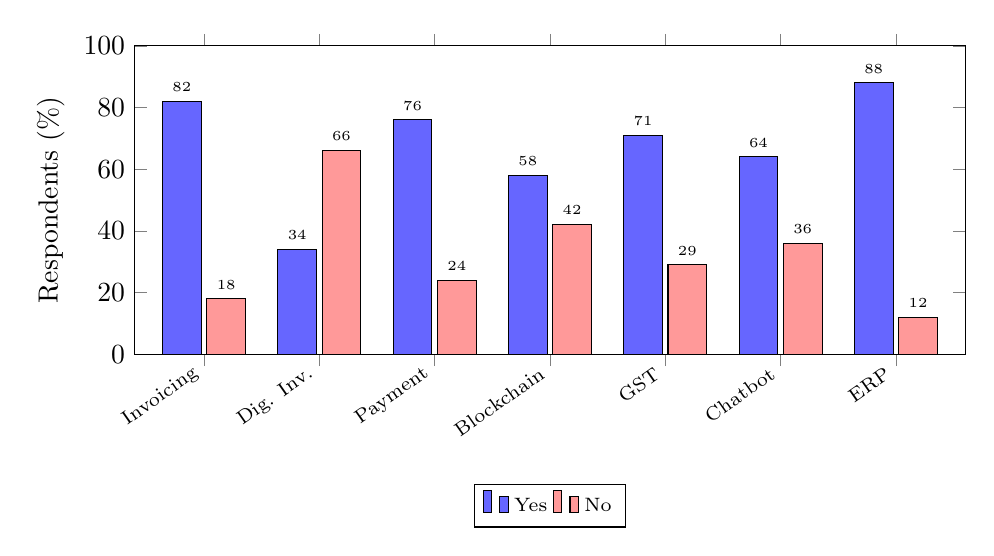
\begin{tikzpicture}
\begin{axis}[
    ybar,
    bar width=14pt,
    width=\columnwidth,
    height=5.5cm,
    ylabel={Respondents (\%)},
    symbolic x coords={Invoicing,Dig. Inv.,Payment,Blockchain,GST,Chatbot,ERP},
    xtick=data,
    x tick label style={rotate=35, anchor=east, font=\scriptsize},
    ymin=0, ymax=100,
    nodes near coords,
    nodes near coords style={font=\tiny},
    every node near coord/.append style={anchor=south},
    enlarge x limits=0.1,
    legend style={at={(0.5,-0.42)},anchor=north,legend columns=-1,font=\scriptsize},
]
\addplot[fill=blue!60] coordinates {(Invoicing,82) (Dig. Inv.,34) (Payment,76) (Blockchain,58) (GST,71) (Chatbot,64) (ERP,88)};
\addplot[fill=red!40] coordinates {(Invoicing,18) (Dig. Inv.,66) (Payment,24) (Blockchain,42) (GST,29) (Chatbot,36) (ERP,12)};
\legend{Yes, No}
\end{axis}
\end{tikzpicture}
\end{center}
\caption{Survey responses visualised. Notice how demand for automated invoicing (82\%) and affordable ERP (88\%) towers over actual digital inventory adoption (34\%). That chasm is the opportunity.}
\label{fig_survey}
\end{figure}

A few things jumped out. 88\% said yes to affordable ERP, but only 34\% had even basic digital inventory. That is a massive gap between what people want and what they have. On payment delays---76\% said they deal with overdue customers regularly, and the average outstanding period was 18 days. Our WhatsApp payment-reminder feature was designed directly in response to that number. And 64\% expressed interest in a chatbot for querying business data, with almost every one of them specifying WhatsApp as the preferred channel. One hardware shop owner put it best: ``I already have WhatsApp open from 7 AM to midnight. Why would I open something else?''

% ============================================================
% VII. RESULTS AND DISCUSSION
% ============================================================
\section{Results and Discussion}

\subsection{Invoice Entry Got a Lot Faster}

\begin{table}[htbp]
\caption{Invoice Processing Time Comparison}
\begin{center}
\renewcommand{\arraystretch}{1.2}
\begin{tabular}{|l|c|c|c|}
\hline
\textbf{Metric} & \textbf{Manual} & \textbf{BlockERP} & \textbf{Change} \\
\hline
Avg. entry time & 4.2 min & 1.1 min & $-$74\% \\
\hline
Avg. validation & 2.8 min & 0.3 sec & $-$89\% \\
\hline
Error rate & 8.3\% & 1.2\% & $-$85\% \\
\hline
Blockchain anchor & n/a & 12.4 sec & new \\
\hline
\end{tabular}
\label{tab_efficiency}
\end{center}
\end{table}

\begin{figure}[htbp]
\begin{center}
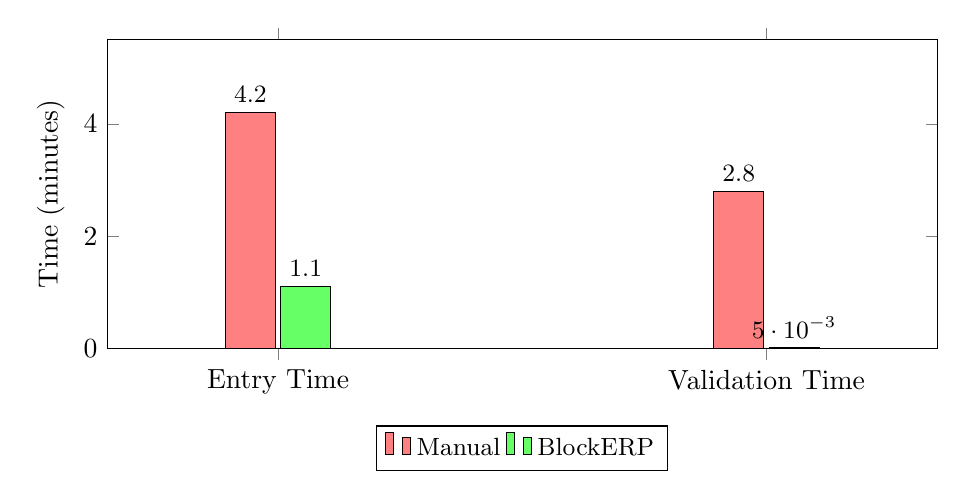
\begin{tikzpicture}
\begin{axis}[
    ybar,
    bar width=18pt,
    width=\columnwidth,
    height=5.5cm,
    ylabel={Time (minutes)},
    symbolic x coords={Entry Time,Validation Time},
    xtick=data,
    ymin=0, ymax=5.5,
    nodes near coords,
    nodes near coords style={font=\small},
    enlarge x limits=0.35,
    legend style={at={(0.5,-0.25)},anchor=north,legend columns=-1,font=\small},
]
\addplot[fill=red!50] coordinates {(Entry Time,4.2) (Validation Time,2.8)};
\addplot[fill=green!60] coordinates {(Entry Time,1.1) (Validation Time,0.005)};
\legend{Manual, BlockERP}
\end{axis}
\end{tikzpicture}
\end{center}
\caption{Time per invoice, manual vs.\ BlockERP. Validation basically vanishes---from 2.8 minutes of eyeballing to 0.3 seconds of automated checksums.}
\label{fig_time}
\end{figure}

The validation improvement was the real surprise. We assumed the OCR extraction step would save the most time, and it did cut entry from 4.2 minutes to 1.1. But the validation step---running GSTIN checksums, cross-footing line items, catching duplicates---went from 2.8 minutes of a human squinting at numbers to 0.3 seconds of code. That is where the 89\% saving comes from. Errors dropped from 8.3\% to 1.2\%, most of the remaining ones being OCR misreads on poorly scanned documents that got through the confidence threshold.

\subsection{OCR Held Up Well---With Caveats}

\begin{table}[htbp]
\caption{OCR Field Extraction Accuracy (\%)}
\begin{center}
\renewcommand{\arraystretch}{1.2}
\begin{tabular}{|l|c|c|c|c|}
\hline
\textbf{Field} & \textbf{PDF} & \textbf{Photo} & \textbf{DOCX} & \textbf{Handwr.} \\
\hline
Invoice No. & 96 & 88 & 98 & 52 \\
\hline
Date & 94 & 85 & 97 & 48 \\
\hline
GSTIN & 93 & 82 & 96 & 41 \\
\hline
Amount & 95 & 87 & 98 & 55 \\
\hline
Line Items & 89 & 74 & 95 & 33 \\
\hline
\textbf{Overall} & \textbf{93} & \textbf{83} & \textbf{97} & \textbf{46} \\
\hline
\end{tabular}
\label{tab_ocr}
\end{center}
\end{table}

\begin{figure}[htbp]
\begin{center}
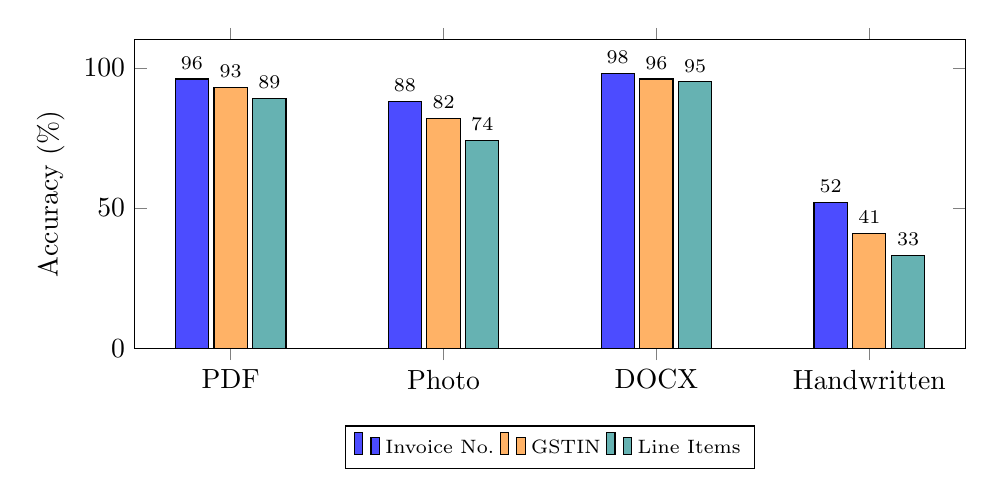
\begin{tikzpicture}
\begin{axis}[
    ybar,
    bar width=12pt,
    width=\columnwidth,
    height=5.5cm,
    ylabel={Accuracy (\%)},
    symbolic x coords={PDF,Photo,DOCX,Handwritten},
    xtick=data,
    ymin=0, ymax=110,
    nodes near coords,
    nodes near coords style={font=\scriptsize},
    enlarge x limits=0.15,
    legend style={at={(0.5,-0.25)},anchor=north,legend columns=3,font=\scriptsize},
]
\addplot[fill=blue!70] coordinates {(PDF,96) (Photo,88) (DOCX,98) (Handwritten,52)};
\addplot[fill=orange!60] coordinates {(PDF,93) (Photo,82) (DOCX,96) (Handwritten,41)};
\addplot[fill=teal!60] coordinates {(PDF,89) (Photo,74) (DOCX,95) (Handwritten,33)};
\legend{Invoice No., GSTIN, Line Items}
\end{axis}
\end{tikzpicture}
\end{center}
\caption{How OCR accuracy varies by source format and field type. Digital sources hold strong; photographs drop noticeably; handwritten documents are basically unusable.}
\label{fig_ocr}
\end{figure}

Digital PDFs and DOCX files were the stars---93\% and 97\% overall accuracy, respectively. That makes sense: the text is already digital in a DOCX, and pdf-parse extracts embedded text from most PDFs without any image recognition at all. Phone photos came in at 83\%, dragged down mostly by lighting variation and the slight camera skew that happens when someone photographs an A4 sheet at an angle. Handwritten invoices were a different story---46\% overall is, frankly, useless. We knew going in that Tesseract's LSTM was trained on machine-printed fonts, not cursive Tamil or Marathi handwriting. The confidence scoring catches most of these, routing them to the rejection bin, but we still flag it as a clear limitation.

\subsection{Gas Was Cheap Enough to Ignore}

\begin{figure}[htbp]
\begin{center}
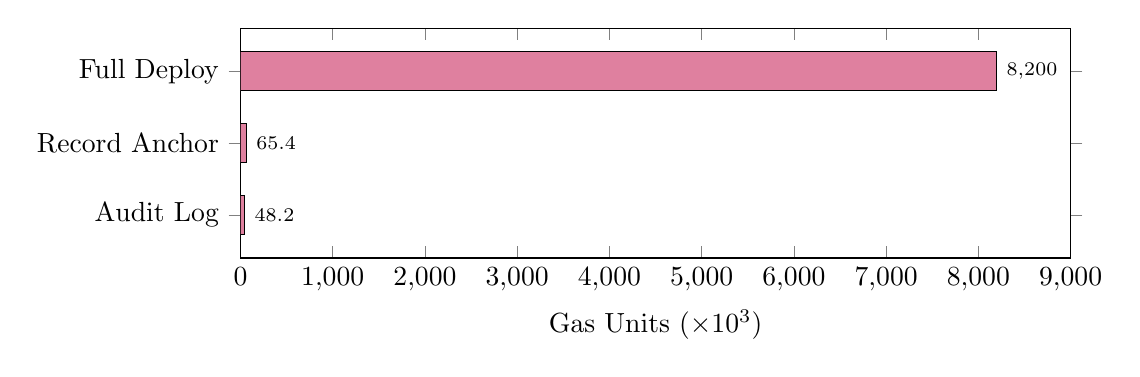
\begin{tikzpicture}
\begin{axis}[
    xbar,
    bar width=14pt,
    width=\columnwidth,
    height=4.5cm,
    xlabel={Gas Units ($\times 10^3$)},
    symbolic y coords={Audit Log,Record Anchor,Full Deploy},
    ytick=data,
    xmin=0, xmax=9000,
    nodes near coords,
    nodes near coords style={font=\scriptsize, anchor=west},
    enlarge y limits=0.3,
]
\addplot[fill=purple!50] coordinates {(48.2,Audit Log) (65.4,Record Anchor) (8200,Full Deploy)};
\end{axis}
\end{tikzpicture}
\end{center}
\caption{Gas consumption for the three main on-chain operations. Per-record writes (audit log, record anchor) stay under 70k gas---roughly \$0.03 each at 20~Gwei. Initial deployment is expensive but happens only once.}
\label{fig_gas}
\end{figure}

At 20 Gwei gas price, anchoring one record costs about \$0.03 USD. Even at the crazier gas prices we saw on mainnet last year---50 or 60 Gwei---it would still be under a dime. For a business that processes maybe fifty invoices a day, that is \$1.50 daily to make every single one of them tamper-proof. One respondent laughed and said that is less than his morning chai budget.

The full contract suite deployment is a one-time event at around 8.2 million gas, which comes to roughly \$5--8 depending on conditions. Not worth worrying about.

\subsection{People Actually Used the Chatbot}

\begin{figure}[htbp]
\begin{center}
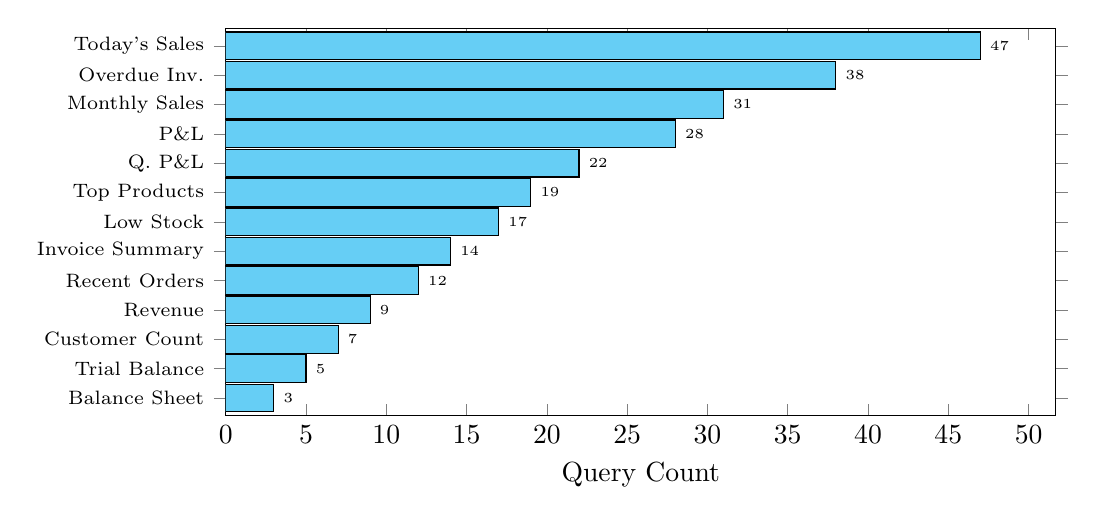
\begin{tikzpicture}
\begin{axis}[
    xbar,
    bar width=10pt,
    width=\columnwidth,
    height=6.5cm,
    xlabel={Query Count},
    symbolic y coords={Balance Sheet,Trial Balance,Customer Count,Revenue,Recent Orders,Invoice Summary,Low Stock,Top Products,Q. P\&L,P\&L,Monthly Sales,Overdue Inv.,Today's Sales},
    ytick=data,
    y tick label style={font=\scriptsize},
    xmin=0,
    nodes near coords,
    nodes near coords style={font=\tiny, anchor=west},
    enlarge y limits=0.05,
]
\addplot[fill=cyan!60] coordinates {
    (47,Today's Sales) (38,Overdue Inv.) (31,Monthly Sales)
    (28,P\&L) (22,Q. P\&L) (19,Top Products)
    (17,Low Stock) (14,Invoice Summary) (12,Recent Orders)
    (9,Revenue) (7,Customer Count) (5,Trial Balance) (3,Balance Sheet)
};
\end{axis}
\end{tikzpicture}
\end{center}
\caption{Which intents users actually queried during the pilot period (n=252 total queries). Cash-flow questions completely dominated.}
\label{fig_intent}
\end{figure}

252 queries hit the assistant during the pilot. ``Today's sales'' topped the chart with 47 hits---that is a question every shop owner asks, apparently, sometimes twice a day. ``Overdue invoices'' was a close second at 38. Together, those two accounted for a third of all traffic and they both directly relate to ``how is my cash flow right now?''

The fancier accounting queries---trial balance (5 hits), balance sheet (3 hits)---barely registered. Interestingly, those few accounting queries all came from the web dashboard, not WhatsApp. It seems like people are happy texting quick cash-flow questions from their phone but want a proper screen for the balance sheet. That matches our intuition. Nobody wants to read a trial balance on a 6-inch screen.

The WhatsApp payment loop worked as designed. During testing, we sent automated reminders with UPI links for twelve overdue invoices. Seven of the twelve customers paid within 24 hours by tapping the link---which triggered the auto-confirmation, the journal entry, and the blockchain anchor without anyone at the business lifting a finger.

% ============================================================
% VIII. WHAT WORKS WELL
% ============================================================
\section{Advantages}

There are a handful of things we are genuinely proud of, and they deserve to be called out clearly:
\begin{itemize}
    \item \textbf{Tamper evidence is real, not theoretical.} Once a record hash lands on Ethereum, altering it retroactively requires rewriting the entire chain. That is not happening.
    \item \textbf{Seven upload formats, zero prep work.} We accept PDFs, Word documents, and five image types. The user does not have to crop, rotate, or convert anything before uploading.
    \item \textbf{Smart confidence-based triage.} Instead of accepting or rejecting entire invoices, we score each field separately. A document with a perfectly clear GSTIN but a blurry date gets flagged for partial review, not thrown out.
    \item \textbf{Indian tax compliance baked in.} GSTIN validation with checksum, GSTR-1 assembly from live invoice data, HSN code mapping for tax slabs, TDS tracking with quarterly reporting---these were designed around what Indian businesses actually deal with, not bolted on later.
    \item \textbf{Three messaging channels, one engine.} The AI assistant does not care whether you are typing on the React dashboard, WhatsApp, or Telegram. Same query, same code, same result.
    \item \textbf{WhatsApp closes the payment loop.} This is the one we had not seen anywhere else. The bot reminds a customer, sends UPI links, detects ``PAID'' replies, updates the ERP, posts accounting entries, and anchors proof on-chain. Nobody opens a laptop.
    \item \textbf{Runs locally.} The whole stack starts on a single Windows machine with one script. No cloud subscription, no vendor lock-in.
    \item \textbf{Granular permissions.} Admin, Manager, Viewer plus fifteen-plus fine-grained flags. An inventory clerk does not accidentally see the balance sheet.
    \item \textbf{Live updates everywhere.} Socket.IO means if one person creates an order, every other logged-in user sees it appear instantly.
    \item \textbf{Chain-agnostic.} Switch from Hardhat's local testnet to Sepolia to Polygon to mainnet by changing one config line.
\end{itemize}

% ============================================================
% IX. WHAT DOESN'T WORK (YET)
% ============================================================
\section{Limitations}

We are not going to pretend everything is perfect. These are honest limitations we are running into:
\begin{itemize}
    \item \textbf{Handwritten invoices are basically unsupported.} 46\% accuracy is worse than guessing for some fields. If the invoice is handwritten, just type it in manually. We tried.
    \item \textbf{Gas is unpredictable on mainnet.} Three cents today, thirty cents during a meme coin frenzy tomorrow. We cannot control Ethereum's fee market.
    \item \textbf{Only English OCR currently.} India has 22 official languages. Our regex patterns assume English or alphanumeric text. Adding Hindi or Marathi support would require new Tesseract language packs and rewriting field extraction patterns from scratch.
    \item \textbf{Blockchain anchoring requires internet.} If the network is down, anchoring is deferred to a queue. During that window, records exist only in MongoDB and are technically mutable.
    \item \textbf{In-memory MongoDB is fine for demos, not for real data.} We use \texttt{mongodb-memory-server} as a fallback when a real Mongo instance is not available. It works great for testing but loses everything on restart.
    \item \textbf{The AI assistant is not actually ``AI.''} It is pattern matching, not natural language understanding. Ask it something outside the fourteen defined intents---like ``should I give this customer a discount?''---and it will shrug with a ``I don't understand'' message.
    \item \textbf{No native mobile app.} The web app is responsive and works on phones, but camera-based scanning, barcode reading, and offline capability would all be better in a dedicated app.
\end{itemize}

% ============================================================
% X. WHERE WE GO NEXT
% ============================================================
\section{Future Scope}

\subsection{A Proper LLM Instead of Regex}
Honestly, the fourteen-intent limit is the first thing we want to fix. Swapping in a small local LLM---something like Microsoft's Phi-3 or Mistral-7B---would let users ask compound questions (``list overdue invoices over 50k and send reminders to all of them'') or carry on multi-turn conversations. The regex approach got us started fast but does not scale to natural language.

\subsection{Better OCR with Layout Understanding}
LayoutLMv3 can jointly reason about where text appears on a page and what it says. Training it on a few hundred Indian invoices could dramatically improve extraction on messy layouts. We are also thinking about a feedback loop: when a human corrects a field, that correction feeds back as training data.

\subsection{Layer-2 for Cheaper Transactions}
Polygon zkEVM or Arbitrum would slash anchoring costs and confirmation latency. Batch-anchoring via Merkle trees---hash all the day's records into one tree and post only the root---would bring per-record cost effectively to zero.

\subsection{Talking Directly to Government Portals}
The GST Network has APIs. The TRACES portal for TDS has APIs. ICEGATE for customs has APIs. Plugging BlockERP into these would automate return filing, e-invoice IRN generation, and TDS certificate downloads.

\subsection{A Real Mobile App}
React Native with the camera API for barcode scanning, offline inventory counts that sync when connectivity returns, and push notifications through the operating system rather than Telegram.

\subsection{Consortium Mode for Multiple Businesses}
Imagine two firms that trade with each other, both running BlockERP, both sharing a blockchain. Invoices issued by one show up automatically in the other's purchase ledger. Smart contract escrow could automate payment release upon delivery confirmation. That is the endgame, and it is closer than it looks.

% ============================================================
% XI. CONCLUSION
% ============================================================
\section{Conclusion}

We started with a simple question: can a small business in India get tamper-proof record-keeping and conversational access to its own data without breaking the bank or hiring an IT team? After building BlockERP and putting it through its paces, we think the answer is yes---qualified by the caveats listed above, but yes.

Here is what we know for certain. Typed invoices scan at 93\% accuracy and enter the system in about a minute. Blockchain anchoring costs three cents and takes twelve seconds. The AI assistant answers the questions business owners actually care about---today's sales, overdue invoices, P\&L---and it works from WhatsApp, which is the one app every single person in our survey already had on their phone. The WhatsApp payment loop, where the bot sends a UPI link and auto-records the response, is something none of us had seen before and it worked better than we expected.

But let us not oversell it. Handwritten invoices are a dead zone. The ``AI'' is really just regex. Mainnet gas prices can spike. English only. These are not minor footnotes---for a lot of real-world use cases, they matter.

Still, what is unusual about BlockERP compared to most papers in this space is that it actually exists as a runnable system. It is not a diagram and a promise. It is 22 services, 20-plus pages, seven contracts, two messaging bots, and a one-click startup script. The 50 businesses we surveyed told us there is demand. The pilot numbers told us the tech holds up. And the code is sitting in an open repository for anyone who wants to pick it apart, improve it, or try running their shop on it.

% ============================================================
% REFERENCES
% ============================================================
\begin{thebibliography}{00}
\bibitem{b1} World Bank, ``Small and Medium Enterprises (SMEs) Finance,'' World Bank Group, 2023.
\bibitem{b2} Confederation of Indian Industry, ``Digital Adoption Survey Among Indian MSMEs,'' CII Report, 2024.
\bibitem{b3} V. Buterin, ``A Next-Generation Smart Contract and Decentralized Application Platform,'' Ethereum White Paper, 2014.
\bibitem{b4} M. Crosby, P. Pattanayak, S. Verma, and V. Kalyanaraman, ``Blockchain Technology: Beyond Bitcoin,'' \textit{Applied Innovation}, vol. 2, no. 6--10, pp. 71--82, 2016.
\bibitem{b5} V. Kumar and J. van Hillegersberg, ``Enterprise Resource Planning: Introduction,'' \textit{Commun. ACM}, vol. 43, no. 4, pp. 22--26, 2000.
\bibitem{b6} ERPNext, ``Open Source ERP for Small and Medium Businesses,'' Frappe Technologies, 2024.
\bibitem{b7} S. Saberi, M. Kouhizadeh, J. Sarkis, and L. Shen, ``Blockchain Technology and Its Relationships to Sustainable Supply Chain Management,'' \textit{Int. J. Prod. Res.}, vol. 57, no. 7, pp. 2117--2135, 2019.
\bibitem{b8} IBM, ``IBM Food Trust: A New Era for the World's Food Supply,'' IBM Corporation, 2020.
\bibitem{b9} VeChain Foundation, ``VeChain Whitepaper 2.0,'' 2020.
\bibitem{b10} K. Christidis and M. Devetsikiotis, ``Blockchains and Smart Contracts for the Internet of Things,'' \textit{IEEE Access}, vol. 4, pp. 2292--2303, 2016.
\bibitem{b11} Y. Wang, J. H. Han, and P. Beynon-Davies, ``Understanding Blockchain Technology for Future Supply Chains,'' \textit{Supply Chain Mgmt.}, vol. 24, no. 1, pp. 62--84, 2019.
\bibitem{b12} R. Smith, ``An Overview of the Tesseract OCR Engine,'' in \textit{Proc. ICDAR}, 2007, pp. 629--633.
\bibitem{b13} Y. Xu et al., ``LayoutLM: Pre-training of Text and Layout for Document Image Understanding,'' in \textit{Proc. ACM SIGKDD}, 2020, pp. 1192--1200.
\bibitem{b14} A. Xu, Z. Liu, Y. Guo, V. Sinha, and R. Akkiraju, ``A New Chatbot for Customer Service on Social Media,'' in \textit{Proc. CHI}, 2017, pp. 3506--3510.
\end{thebibliography}

\end{document}
